\section{Data Processing}
    All data was saved as a \texttt{.txt} file. We also did some additional work to visualize the data to make sure it was being processed correctly.
    \subsection{Factory Region}
        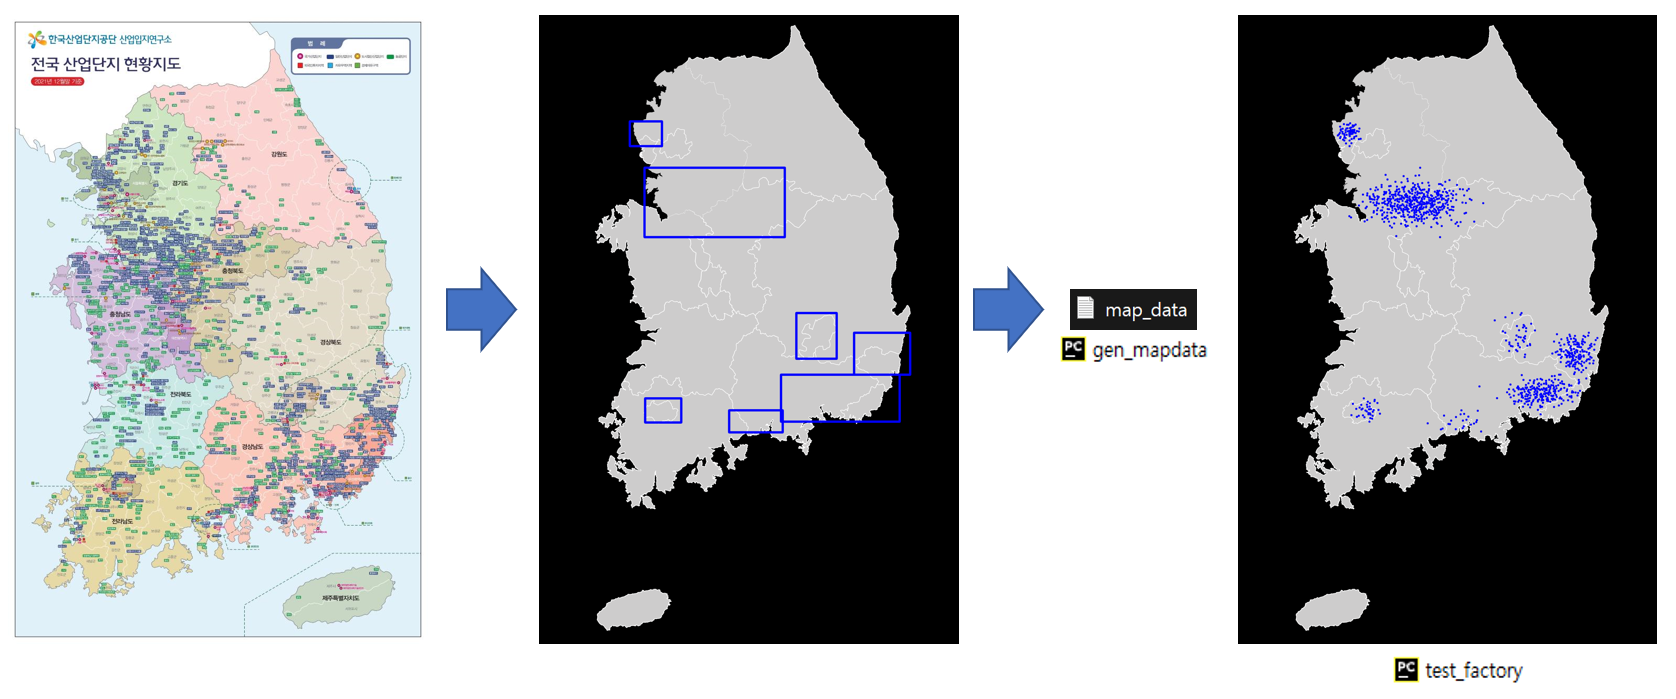
\includegraphics[scale = 0.7]{factoryregion.png}\\
        The locations of the factories were randomized according to a Gaussian distribution in areas with a high concentration of factories, such as industrial parks. As shown in the image above, the factory concentration areas were marked with squares and random dots were placed on them.\\
        When saving to a text file, each pixel was saved as 0 for \texttt{sea}, 1 for \texttt{land}, and 2 for \texttt{factory}.
    \subsection{Wind}
        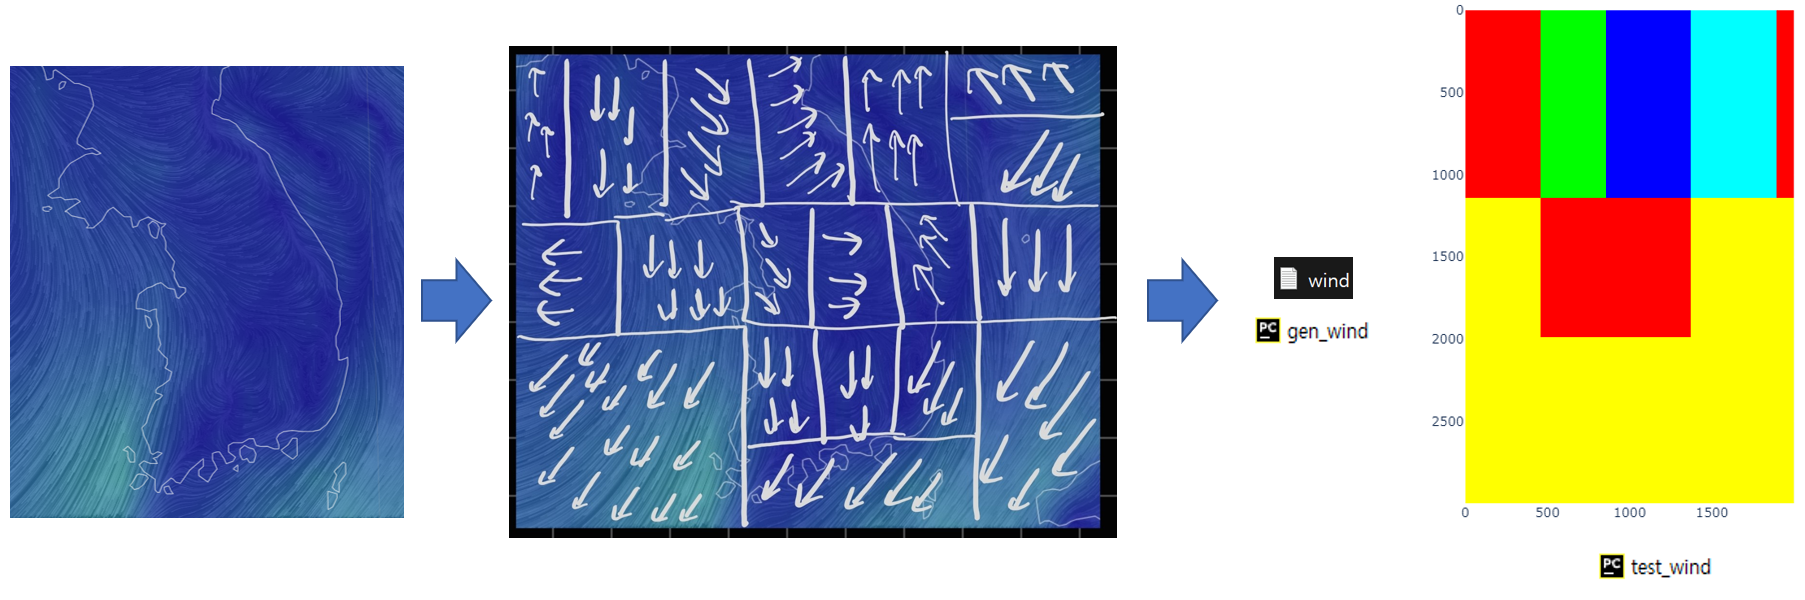
\includegraphics[scale = 0.7]{wind.png}\\
        The wind direction is based on the real-time wind direction given on the \texttt{nullschool} website. Since the exact direction of each pixel was not available, the wind direction was divided into 8 main directions and areas were seperated based on the main directions.\\
        In the text file, each pixel was assigned a number from 1 to 8 depending on the direction.
    \subsection{Particulate matter}
        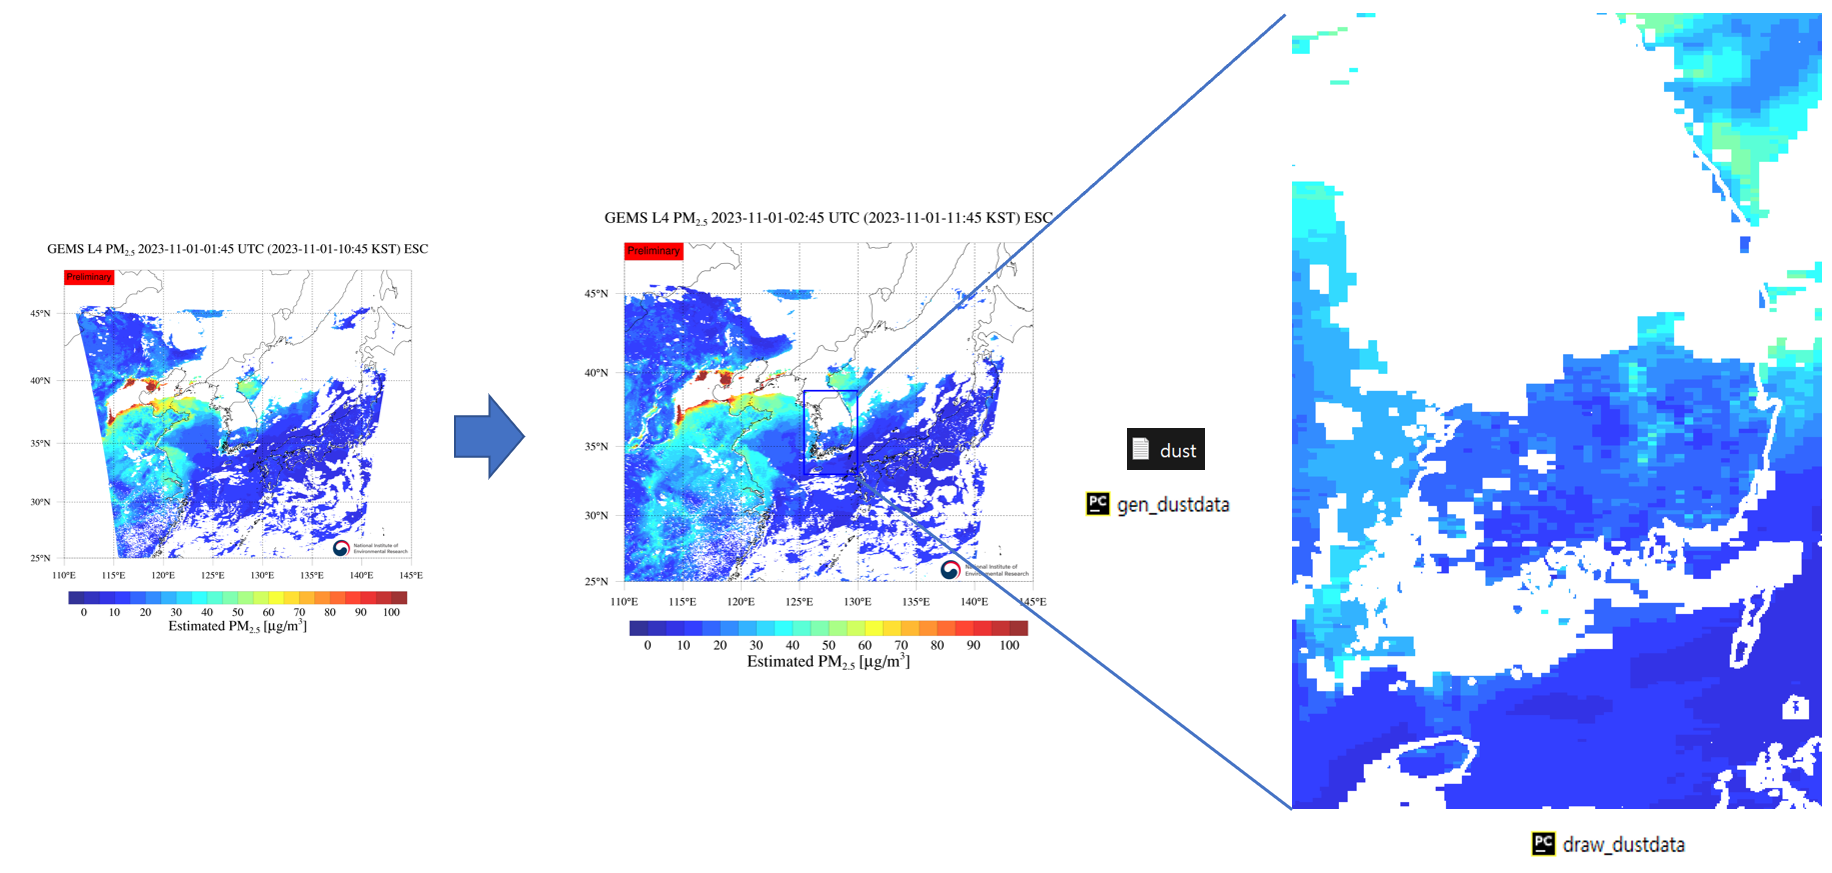
\includegraphics[scale = 0.7]{particulatematter.png}\\
        Initial particulate matter concentration data was obtained from the National Center for Environmental Science. However, the data was given in the form of map colors rather than numbers, so we scaled it as shown in the image above and used the RGB values to get the concentration of fine dust by pixel location.\\
        Each concentration was multiplied by 1000 for smooth integer operations.